\section{Utente Autenticato}

Di seguito vengono elencati i casi d'uso per l'utente autenticato.

\subsubsection{UC-U8}

    \begin{figure}[H]
      \begin{center}
        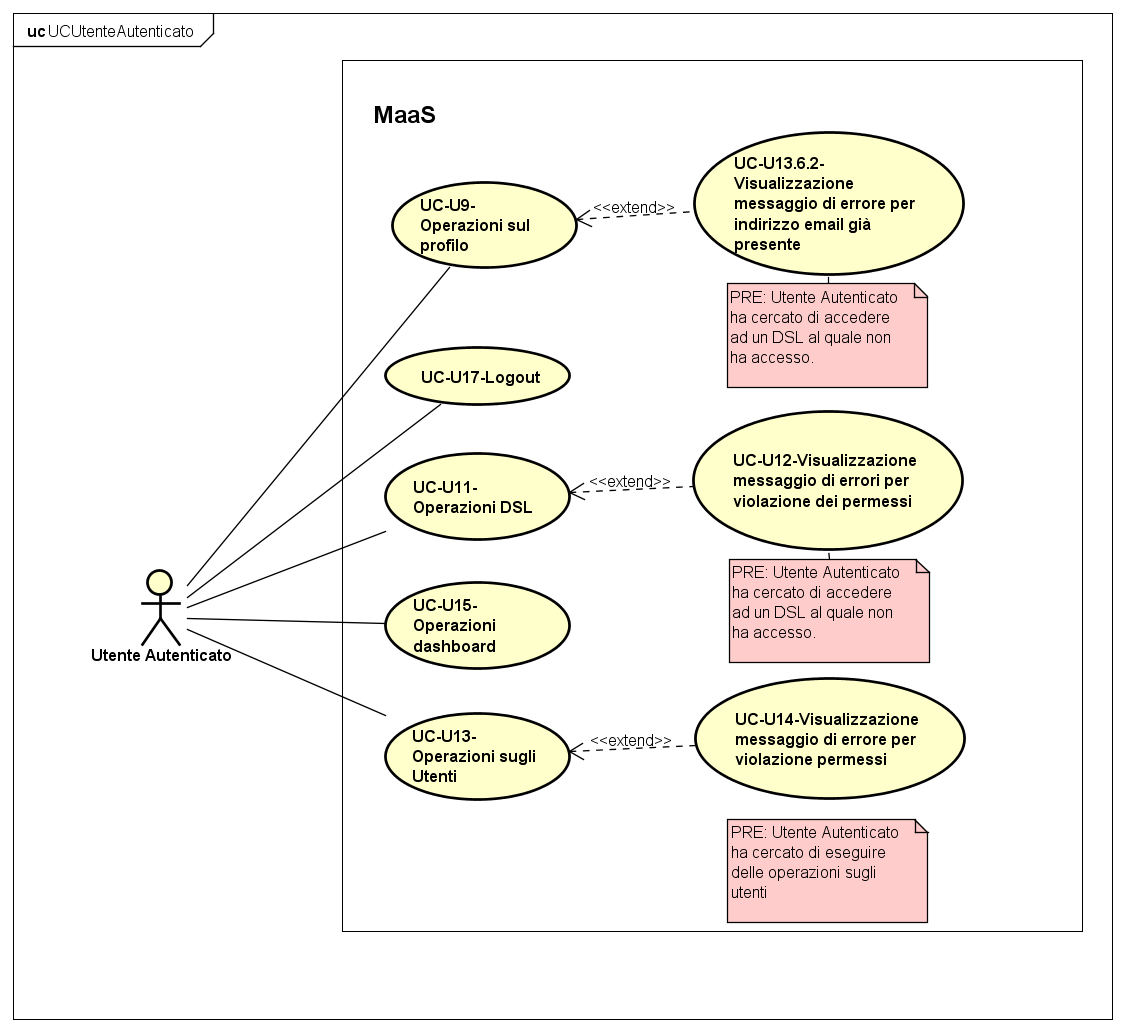
\includegraphics[width=12cm]{res/img/UCUtenti/UCUtenteA/UC-U8-OperazioniUtenteAutenticato}
      \caption{UC-U8 - Operazioni dell'utente autenticato}
      \end{center} 
    \end{figure}    
    
    %Tabella 
    \begin{center}
      \bgroup
      \def\arraystretch{1.8}     
      \begin{longtable}{  p{3.5cm} | p{8cm} } 
        
        \hline
        \multicolumn{2}{ | c | }{ \cellcolor[gray]{0.9} \textbf{UC-U8 - Operazioni dell'utente autenticato}} \\ 
        \hline
        
        \textbf{Attori Primari} & Utente autenticato \\ 
        \textbf{Scopo e Descrizione} & L’utente autenticato può: modificare il proprio profilo, effettuare delle operazioni nella pagina Dashboard, effettuare delle operazioni di creazione/modifica/esecuzione del DSL (a seconda dei suoi permessi) e gestire altri utenti (quest'ultima funzionalità è riservata ad un ruolo superiore o uguale all'admin). \\ 
        
        \textbf{Precondizioni}  & L’applicazione MaaS è funzionante e pronta all'uso. L'utente autenticato può accedere alla propria pagina Dashboard. \\ 
        
        \textbf{Postcondizioni} & L'applicazione ha eseguito le azioni richieste dall'utente. \\ 
        \textbf{Flusso Principale} & 1. L'utente modifica il proprio profilo (UC-U9)
        
2. L'utente effettua delle operazioni nella pagina Dashboard (UC-U15)

3. L'utente effettua delle operazioni di creazione/modifica/esecuzione del DSL (a seconda dei suoi permessi) (UC-U11)

4. L'utente gestisce altri utenti (quest'ultima funzionalità è riservata ad un ruolo superiore o uguale all'admin) (UC-U13) \\
        \textbf{Estensioni} & 1. L'utente autenticato visualizza un messaggio di errore nella proceduro di modifica del profilo dovuto all'inserimento di un indirizzo email già presente (UC-U13.6.2)
        
2. L'utente autenticato visualizza un messaggio di errore durante le operazioni effettuate sul DSL dovuto alla violazione dei permessi (UC-U12)

3. L'utente autenticato visualizza un messaggio di errore durante le operazioni sugli utenti dovute alla violazione dei permessi (UC-u14) \\
        \textbf{Inclusioni} & Nessuna \\
      \end{longtable}
      \egroup
    \end{center} 


\subsubsection{UC-U9}

    \begin{figure}[H]
      \begin{center}
        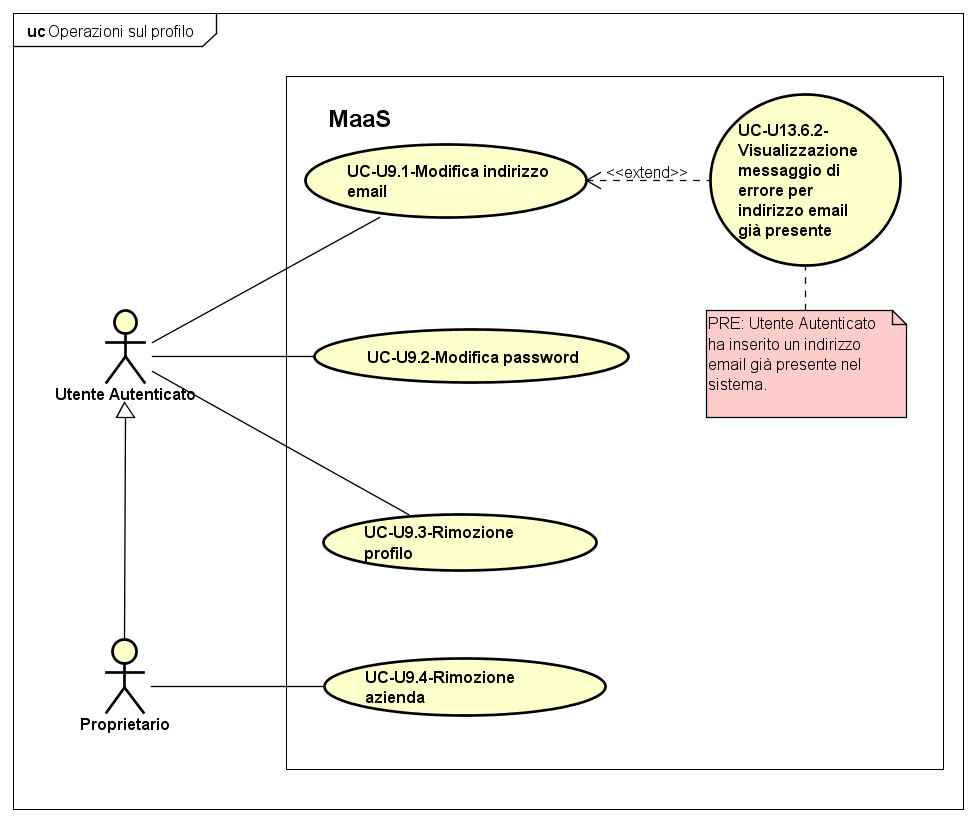
\includegraphics[width=12cm]{res/img/UCUtenti/UCUtenteA/UC-U9- Operazioni sul profilo/Operazioni sul profilo}
      \caption{UC-U9 - Operazioni sul profilo}
      \end{center} 
    \end{figure}    
    
    %Tabella 
    \begin{center}
      \bgroup
      \def\arraystretch{1.8}     
      \begin{longtable}{  p{3.5cm} | p{8cm} } 
        
        \hline
        \multicolumn{2}{ | c | }{ \cellcolor[gray]{0.9} \textbf{UC-U9 - Operazioni sul profilo}} \\ 
        \hline
        
        \textbf{Attori Primari} & Utente autenticato \\ 
        \textbf{Scopo e Descrizione} & L'utente autenticato visualizza la pagina per apportare modifiche al profilo personale. Può decidere di: modificare l'indirizzo email, la password, o rimuovere il profilo. \\ 
        
        \textbf{Precondizioni}  & L’applicazione MaaS è funzionante e pronta all'uso. L'utente autenticato può accedere alla propria pagina Dashboard. \\ 
        
        \textbf{Postcondizioni} & Le (eventuali) modifiche del profilo richieste dall'utente sono state apportate. \\ 
        \textbf{Flusso Principale} & 1. L'utente autenticato modifica il proprio indirizzo email (UC-U9.1)
        
2. L'utente autenticato modifica la propria password (UC-U9.2)

3. L'utente autenticato rimuove il suo profilo/account (UC-U9.3)

4. Il proprietario rimuove la propria azienda (UC-U9.4) \\
        \textbf{Estensioni} & 1. L'utente visualizza un messaggio di errore durante la modifica dell'email dovuto all'inserimento di un indirizzo email già presente. \\
        \textbf{Inclusioni} & Nessuna \\
      \end{longtable}
      \egroup
    \end{center} 

\subsubsection{UC-U9.1}
 

    \begin{figure}[H]
      \begin{center}
        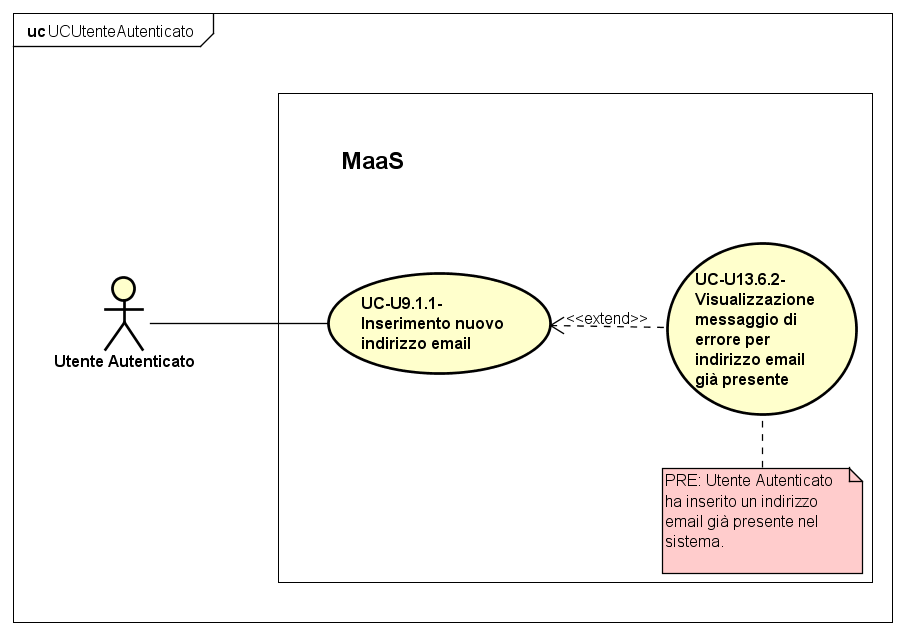
\includegraphics[width=12cm]{res/img/UCUtenti/UCUtenteA/UC-U9.1-Modifica indirizzo email/UC-U9.1-Modifica indirizzo email}
      \caption{UC-U9.1 - Modifica indirizzo email}
      \end{center} 
    \end{figure}

    %Tabella 
    \begin{center}
      \bgroup
      \def\arraystretch{1.8}     
      \begin{longtable}{  p{3.5cm} | p{8cm} } 
        
        \hline
        \multicolumn{2}{ | c | }{ \cellcolor[gray]{0.9} \textbf{UC-U9.1 - Modifica indirizzo email}} \\ 
        \hline
        
        \textbf{Attori Primari} & Utente autenticato \\ 
        \textbf{Scopo e Descrizione} & L'utente autenticato può modificare il proprio indirizzo email nella procedura di modifica del profilo. \\ 
        
        \textbf{Precondizioni}  & L'utente autenticato ha visualizzato la pagina di modifica del profilo. \\ 
        
        \textbf{Postcondizioni} & L'utente autenticato dispone di un nuovo indirizzo email, che sostituisce il vecchio. \\ 
        \textbf{Flusso Principale} & 1. L'utente autenticato inserisce un nuovo indirizzo email (UC-U9.1.1) \\
        \textbf{Estensioni} & 1. L'utente autenticato visualizza un messaggio di errore causato dall'inserimento di un indirizzo email già presente (UC-U13.6.2) \\
        \textbf{Inclusioni} & Nessuna
      \end{longtable}
      \egroup
    \end{center}
    
\subsubsection{UC-U9.1.1}

    %Tabella 
    \begin{center}
      \bgroup
      \def\arraystretch{1.8}     
      \begin{longtable}{  p{3.5cm} | p{8cm} } 
        
        \hline
        \multicolumn{2}{ | c | }{ \cellcolor[gray]{0.9} \textbf{UC-U9.1.1 - Inserimento di un nuovo indirizzo email}} \\ 
        \hline
        
        \textbf{Attori Primari} & Utente autenticato \\ 
        \textbf{Scopo e Descrizione} & L'utente autenticato può inserire un nuovo indirizzo email nella procedura di modifica del profilo. \\ 
        
        \textbf{Precondizioni}  & L'utente autenticato ha visualizzato la pagina di modifica del profilo. \\ 
        
        \textbf{Postcondizioni} & L'utente autenticato ha inserito un nuovo indirizzo email. \\ 
        \textbf{Flusso Principale} & Nessuno \\
        \textbf{Estensioni} & Nessuna \\
        \textbf{Inclusioni} & Nessuna
      \end{longtable}
      \egroup
    \end{center}
\subsubsection{UC-U13.6.2}

    %Tabella 
    \begin{center}
      \bgroup
      \def\arraystretch{1.8}     
      \begin{longtable}{  p{3.5cm} | p{8cm} } 
        
        \hline
        \multicolumn{2}{ | c | }{ \cellcolor[gray]{0.9} \textbf{UC-U13.6.2 - Visualizzazione di messaggio di errore per indirizzo email già presente}} \\ 
        \hline
        
        \textbf{Attori Primari} & Utente autenticato \\ 
        \textbf{Scopo e Descrizione} & L'utente autenticato visualizza un messaggio di errore durante la procedura di modifica del profilo causato dall'inserimento di un indirizzo email già presente in MaaS. \\ 
        
        \textbf{Precondizioni}  & L'utente autenticato ha inserito un indirizzo email già presente nel sistema. \\ 
        
        \textbf{Postcondizioni} & L'utente autenticato ha visualizzato il messaggio di errore. \\ 
        \textbf{Flusso Principale} & Nessuno \\
        \textbf{Estensioni} & Nessuna \\
        \textbf{Inclusioni} & Nessuna
      \end{longtable}
      \egroup
    \end{center}
\subsubsection{UC-U9.2}
 

    \begin{figure}[H]
      \begin{center}
        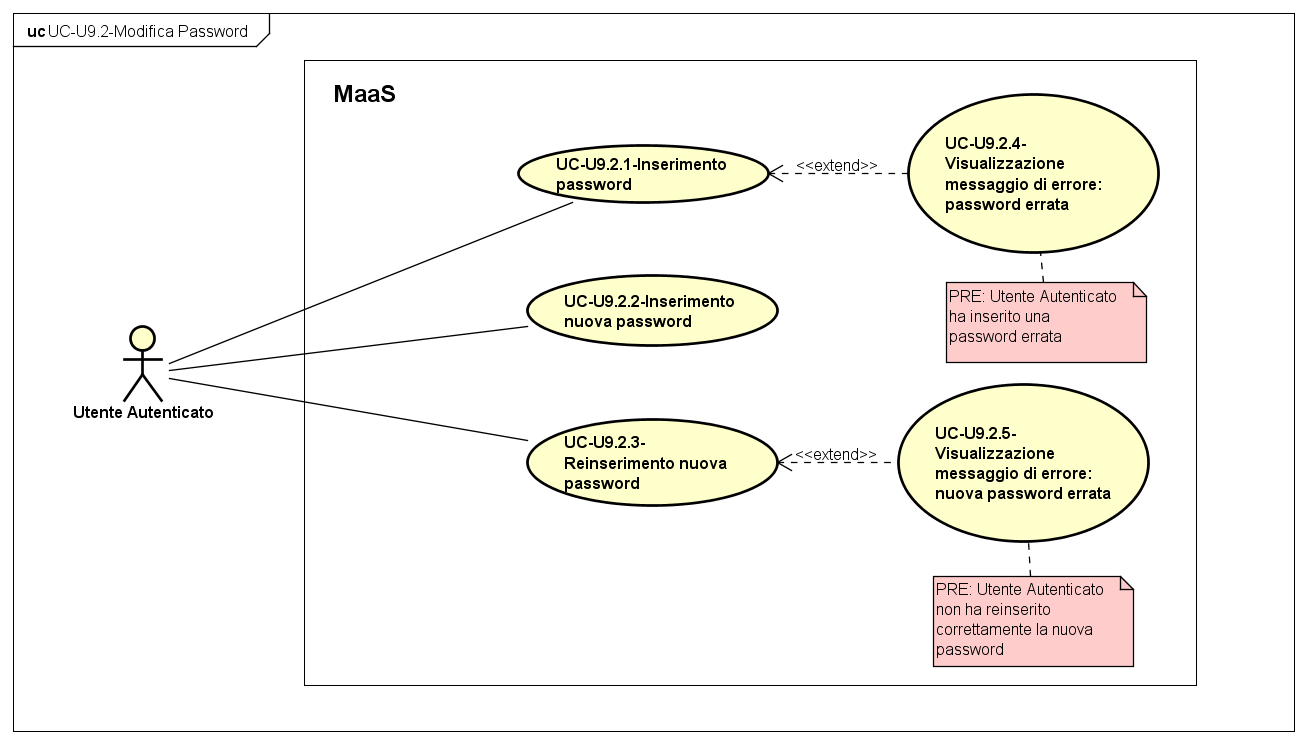
\includegraphics[width=12cm]{res/img/UCUtenti/UCUtenteA/UC-U9.2-Modifica password/UC-U9.2-Modifica password}
      \caption{UC-U9.2 - Modifica password}
      \end{center} 
    \end{figure}

    %Tabella 
    \begin{center}
      \bgroup
      \def\arraystretch{1.8}     
      \begin{longtable}{  p{3.5cm} | p{8cm} } 
        
        \hline
        \multicolumn{2}{ | c | }{ \cellcolor[gray]{0.9} \textbf{UC-U9.2 - Modifica password}} \\ 
        \hline
        
        \textbf{Attori Primari} & Utente autenticato \\ 
        \textbf{Scopo e Descrizione} & L'utente autenticato può modificare la password del proprio account. \\ 
        
        \textbf{Precondizioni}  & L'utente autenticato ha visualizzato la pagina di modifica del profilo. \\ 
        
        \textbf{Postcondizioni} & L'utente autenticato ha sostituito la password precedente con quella da lui inserita. \\ 
        \textbf{Flusso Principale} & 1. L'utente autenticato inserisce la password corrente (UC-U9.2.1)
        
2. L'utente autenticato inserisce una nuova password (UC-U9.2.2)

3. L'utente autenticato re-inserisce la nuova password (UC-U9.2.3) \\
        \textbf{Estensioni} & 1. L'utente autenticato visualizza un messaggio di errore dovuto all'inserimento di una password errata (UC-U9.2.4)
        
2. L'utente autenticato visualizza un messaggio di errore dovuto al reinserimento della nuova password (non corrisponde alla nuova password già inserita) (UC-U9.2.5) \\
        \textbf{Inclusioni} & Nessuna
      \end{longtable}
      \egroup
    \end{center}
    
\subsubsection{UC-U9.2.1}

    %Tabella 
    \begin{center}
      \bgroup
      \def\arraystretch{1.8}     
      \begin{longtable}{  p{3.5cm} | p{8cm} } 
        
        \hline
        \multicolumn{2}{ | c | }{ \cellcolor[gray]{0.9} \textbf{UC-U9.2.1 - Inserimento Password}} \\ 
        \hline
        
        \textbf{Attori Primari} & Utente autenticato \\ 
        \textbf{Scopo e Descrizione} & L'utente autenticato inserisce la password corrente. \\ 
        
        \textbf{Precondizioni}  & L'utente autenticato ha visualizzato la pagina di modifica del profilo. \\ 
        
        \textbf{Postcondizioni} & L'utente autenticato ha inserito la propria password. \\ 
        \textbf{Flusso Principale} & Nessuno \\
        \textbf{Estensioni} & Nessuna \\
        \textbf{Inclusioni} & Nessuna
      \end{longtable}
      \egroup
    \end{center}
\subsubsection{UC-U9.2.2}

    %Tabella 
    \begin{center}
      \bgroup
      \def\arraystretch{1.8}     
      \begin{longtable}{  p{3.5cm} | p{8cm} } 
        
        \hline
        \multicolumn{2}{ | c | }{ \cellcolor[gray]{0.9} \textbf{UC-U9.2.2 - Inserimento nuova password}} \\ 
        \hline
        
        \textbf{Attori Primari} & Utente autenticato \\ 
        \textbf{Scopo e Descrizione} & L'utente autenticato inserisce una nuova password in sostituzione di quella precedente.  \\ 
        
        \textbf{Precondizioni}  & L'utente autenticato ha visualizzato la pagina di modifica del profilo. \\ 
        
        \textbf{Postcondizioni} & L'utente autenticato ha inserito una nuova password. \\ 
        \textbf{Flusso Principale} & Nessuno \\
        \textbf{Estensioni} & Nessuna \\
        \textbf{Inclusioni} & Nessuna
      \end{longtable}
      \egroup
    \end{center}
	
\subsubsection{UC-U9.2.3}

    %Tabella 
    \begin{center}
      \bgroup
      \def\arraystretch{1.8}     
      \begin{longtable}{  p{3.5cm} | p{8cm} } 
        
        \hline
        \multicolumn{2}{ | c | }{ \cellcolor[gray]{0.9} \textbf{UC-U9.2.3 - Reinserimento password}} \\ 
        \hline
        
        \textbf{Attori Primari} & Utente autenticato \\ 
        \textbf{Scopo e Descrizione} & L'utente autenticato ripete l'inserimento della nuova password. \\ 
        
        \textbf{Precondizioni}  & L'utente autenticato ha precedentemente inserito la nuova password. (UC-U9.2.2) \\ 
        
        \textbf{Postcondizioni} & L'utente autenticato ha completato la procedura di cambiamento della password. La nuova password inserita ha sostituito la password precedente. \\ 
        \textbf{Flusso Principale} & Nessuno \\
        \textbf{Estensioni} & Nessuna \\
        \textbf{Inclusioni} & Nessuna
      \end{longtable}
      \egroup
    \end{center}
	
\subsubsection{UC-U9.2.4}

    %Tabella 
    \begin{center}
      \bgroup
      \def\arraystretch{1.8}     
      \begin{longtable}{  p{3.5cm} | p{8cm} } 
        
        \hline
        \multicolumn{2}{ | c | }{ \cellcolor[gray]{0.9} \textbf{UC-U9.2.4 - Visualizzazione messaggio di errore: password errata}} \\ 
        \hline
        
        \textbf{Attori Primari} & Utente autenticato \\ 
        \textbf{Scopo e Descrizione} & L'utente autenticato visualizza un messaggio di errore durante procedura di modifica del profilo dovuto all'inserimento di una password errata. \\ 
        
        \textbf{Precondizioni}  & L'utente autenticato ha inserito una password errata nella procedura di cambio della password. \\ 
        
        \textbf{Postcondizioni} & L'utente autenticato ha visualizzato il messaggio di errore. \\ 
        \textbf{Flusso Principale} & Nessuno \\
        \textbf{Estensioni} & Nessuna \\
        \textbf{Inclusioni} & Nessuna
      \end{longtable}
      \egroup
    \end{center}

\subsubsection{UC-U9.2.5}

    %Tabella 
    \begin{center}
      \bgroup
      \def\arraystretch{1.8}     
      \begin{longtable}{  p{3.5cm} | p{8cm} } 
        
        \hline
        \multicolumn{2}{ | c | }{ \cellcolor[gray]{0.9} \textbf{UC-U9.2.5 - Visualizzazione messaggio di errore: nuova password errata}} \\ 
        \hline
        
        \textbf{Attori Primari} & Utente autenticato \\ 
        \textbf{Scopo e Descrizione} & L'utente autenticato visualizza un messaggio di errore dovuto al reinserimento errato della nuova password (la nuova password è diversa da quella inserita la prima volta). \\ 
        
        \textbf{Precondizioni}  & L'utente autenticato non ha reinserito correttamente la nuova password. \\ 
        
        \textbf{Postcondizioni} & L'utente autenticato ha visualizzato il messaggio di errore. \\ 
        \textbf{Flusso Principale} & Nessuno \\
        \textbf{Estensioni} & Nessuna \\
        \textbf{Inclusioni} & Nessuna
      \end{longtable}
      \egroup
    \end{center}
    
\subsubsection{UC-U15}
 

    \begin{figure}[H]
      \begin{center}
        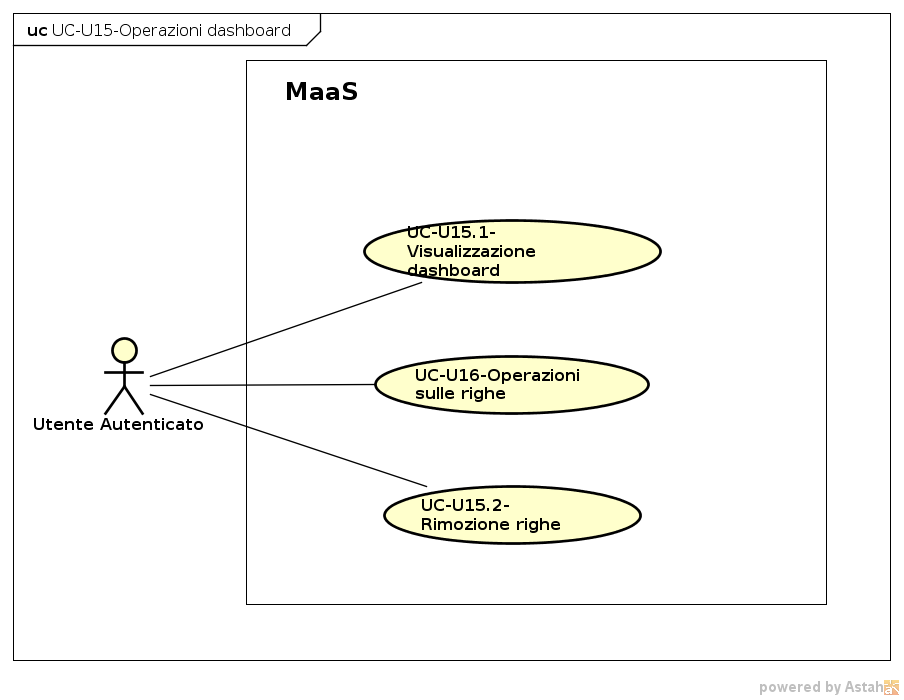
\includegraphics[width=12cm]{res/img/UCUtenti/UCUtenteA/UC-U15-Operazioni-dashboard/UC-U15-Operazioni-dashboard}
      \caption{UC-U15 - Operazioni dashboard}
      \end{center} 
    \end{figure}

    %Tabella 
    \begin{center}
      \bgroup
      \def\arraystretch{1.8}     
      \begin{longtable}{  p{3.5cm} | p{8cm} } 
        
        \hline
        \multicolumn{2}{ | c | }{ \cellcolor[gray]{0.9} \textbf{UC-U15 - Operazioni dashboard}} \\ 
        \hline
        
        \textbf{Attori Primari} & Utente autenticato \\ 
        \textbf{Scopo e Descrizione} & L'utente autenticato può: visualizzare la dashboard, effettuare delle operazioni sulle righe della dashboard, rimuovere le righe della dashboard. \\ 
        
        \textbf{Precondizioni}  & L'utente autenticato si trova nella pagina iniziale dashboard. \\ 
        
        \textbf{Postcondizioni} & L'applicazione MaaS ha eseguito le operazioni richieste dall'utente. \\ 
        \textbf{Flusso Principale} & 1. L'utente autenticato visualizza la dashboard (UC-U15.1)
        
2. L'utente autenticato effettua delle operazioni sulle righe (UC-U16)

3. L'utente autenticato rimuove delle righe dalla dashboard (UC-U15.2) \\
        \textbf{Estensioni} & Nessuna \\
        \textbf{Inclusioni} & Nessuna
      \end{longtable}
      \egroup
    \end{center}

\subsubsection{UC-U16}

    \begin{figure}[H]
      \begin{center}
        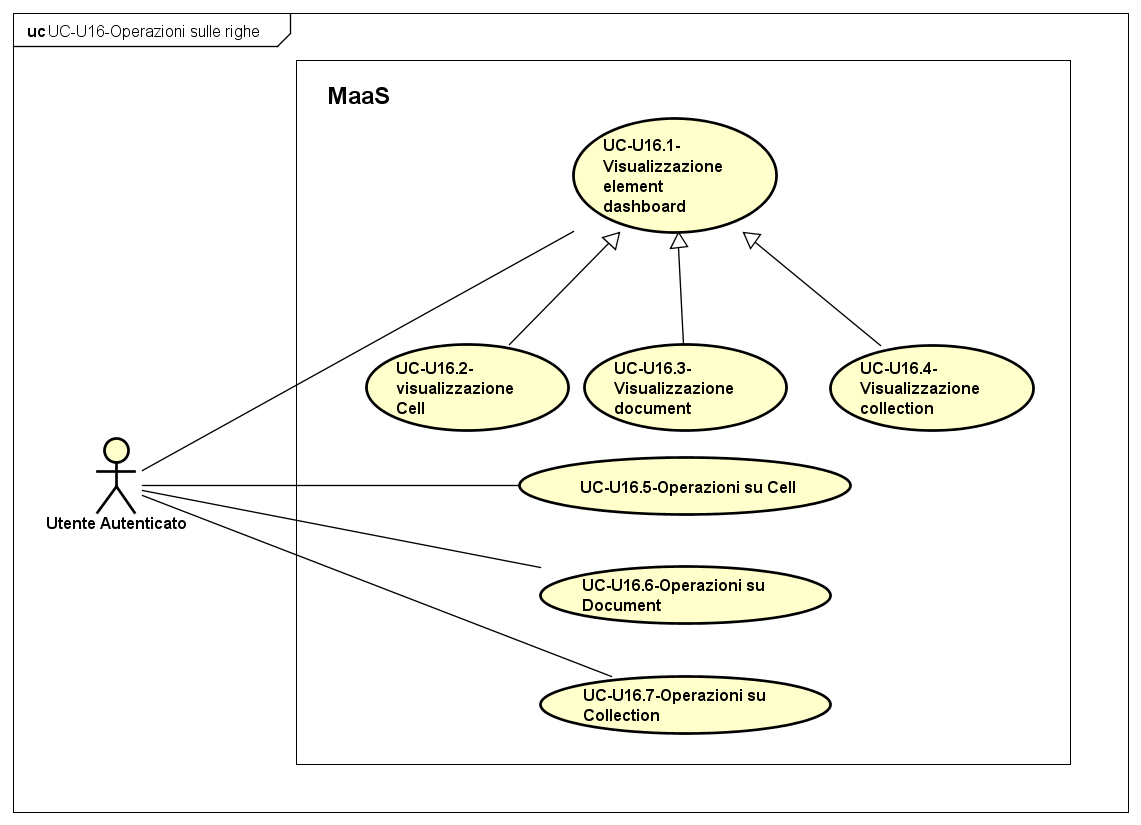
\includegraphics[width=12cm]{res/img/UCUtenti/UCUtenteA/UC-U16-Operazioni_sulle_righe/UC-U16-Operazioni_sulle_righe}
      \caption{UC-U16 - Operazioni sulle righe della dashboard}
      \end{center} 
    \end{figure}

    %Tabella 
    \begin{center}
      \bgroup
      \def\arraystretch{1.8}     
      \begin{longtable}{  p{3.5cm} | p{8cm} } 
        
        \hline
        \multicolumn{2}{ | c | }{ \cellcolor[gray]{0.9} \textbf{UC-U16 - Operazioni sulle righe della dashboard}} \\ 
        \hline
        
        \textbf{Attori Primari} & Utente autenticato \\ 
        \textbf{Scopo e Descrizione} & L'utente autenticato può eseguire le seguenti azioni sulle righe della dashboard: visualizzare un elemento di una riga (che può essere una cell, un document o una collection) oppure effettuare un'operazione su un elemento di una riga. \\ 
        
        \textbf{Precondizioni}  & L'utente autenticato ha visualizzato la pagina iniziale dashboard. \\ 
        
        \textbf{Postcondizioni} & L'applicazione MaaS ha eseguito le operazioni sulle righe della dashboard richieste dall'utente autenticato. \\ 
        \textbf{Flusso Principale} & 1. Visualizzazione element dashboard
        
1.1 L'utente visualizza una cell (UC-U16.1)

1.2 L'utente visualizza un document (UC-U16.1)

1.3 L'utente visualizza una collection (UC-U16.1)

2. L'utente desidera effettuare un'operazione su una riga

2.1 L'utente effettua un'operazione su una cell (UC-U16.4)

2.2 L'utente effettua un'operazione su un document (UC-U16.5)

2.3 L'utente effettua un'operazione su una collection (UC-U16.6) \\
        \textbf{Estensioni} & Nessuna \\
        \textbf{Inclusioni} & Nessuna
      \end{longtable}
      \egroup
    \end{center}

\subsubsection{UC-U15.1}

    %Tabella 
    \begin{center}
      \bgroup
      \def\arraystretch{1.8}     
      \begin{longtable}{  p{3.5cm} | p{8cm} } 
        
        \hline
        \multicolumn{2}{ | c | }{ \cellcolor[gray]{0.9} \textbf{UC-U15.1 - Visualizzazione dashboard}} \\ 
        \hline
        
        \textbf{Attori Primari} & Utente autenticato \\ 
        \textbf{Scopo e Descrizione} & L'utente autenticato visualizza la dashboard nella pagina dashboard. \\ 
        
        \textbf{Precondizioni}  & L'utente si trova nella pagina dashboard. \\ 
        
        \textbf{Postcondizioni} & L'utente ha visualizzato la propria dashboard. \\ 
        \textbf{Flusso Principale} & Nessuno \\
        \textbf{Estensioni} & Nessuna \\
        \textbf{Inclusioni} & Nessuna
      \end{longtable}
      \egroup
    \end{center}
    
\subsubsection{UC-U16.1}

    %Tabella 
    \begin{center}
      \bgroup
      \def\arraystretch{1.8}     
      \begin{longtable}{  p{3.5cm} | p{8cm} } 
        
        \hline
        \multicolumn{2}{ | c | }{ \cellcolor[gray]{0.9} \textbf{UC-U16.1 - Visualizzazione element dashboard}} \\ 
        \hline
        
        \textbf{Attori Primari} & Utente autenticato \\ 
        \textbf{Scopo e Descrizione} & L'utente autenticato sceglie di visualizzare un element da una riga della dahboard (che può essere una cell, un document o una collection). \\ 
        
        \textbf{Precondizioni}  & L'utente autenticato ha visualizzato un element della dashboard. \\ 
        
        \textbf{Postcondizioni} & L'utente autenticato ha visualizzato un element di una riga della dashboard. \\ 
        \textbf{Flusso Principale} & Nessuno \\
        \textbf{Estensioni} & Nessuna \\
        \textbf{Inclusioni} & Nessuna
      \end{longtable}
      \egroup
    \end{center}

\newpage